%\info{Ben, Andrzej, Jesse, Gregory, Grigorios, Frederic}

\subsection{Extraction of Theory Templates}

	Theory Templates.

	Ben is doing this.

	Current best NNLO + NLO for dijets, but for time, drop both first Ns
 
 Can do NLO + LO on days timescale (even if theory uncertainty is too large)

 Right now, assume known quark/gluon function, relax later.


\subsection{Estimate of Experimental Resolution}

	Parametrized Experimental Resolution? Fig.~\ref{fig:expfit}.

	Ben has a toy simulation
	Resolution achievable, uncertainty?
	How to we think this will be done in this study (can we use fast simulation, or parametrization?)
	Statistical uncertainties at high pT?
	Pileup:  there are studies of this with current level of pileup, not a big deal yet

	Uncertainty worse at low and high mass, need to derive parametrized uncertainty
	
	Trade off with pT (rate versus NP control)

\begin{figure}
\begin{center}
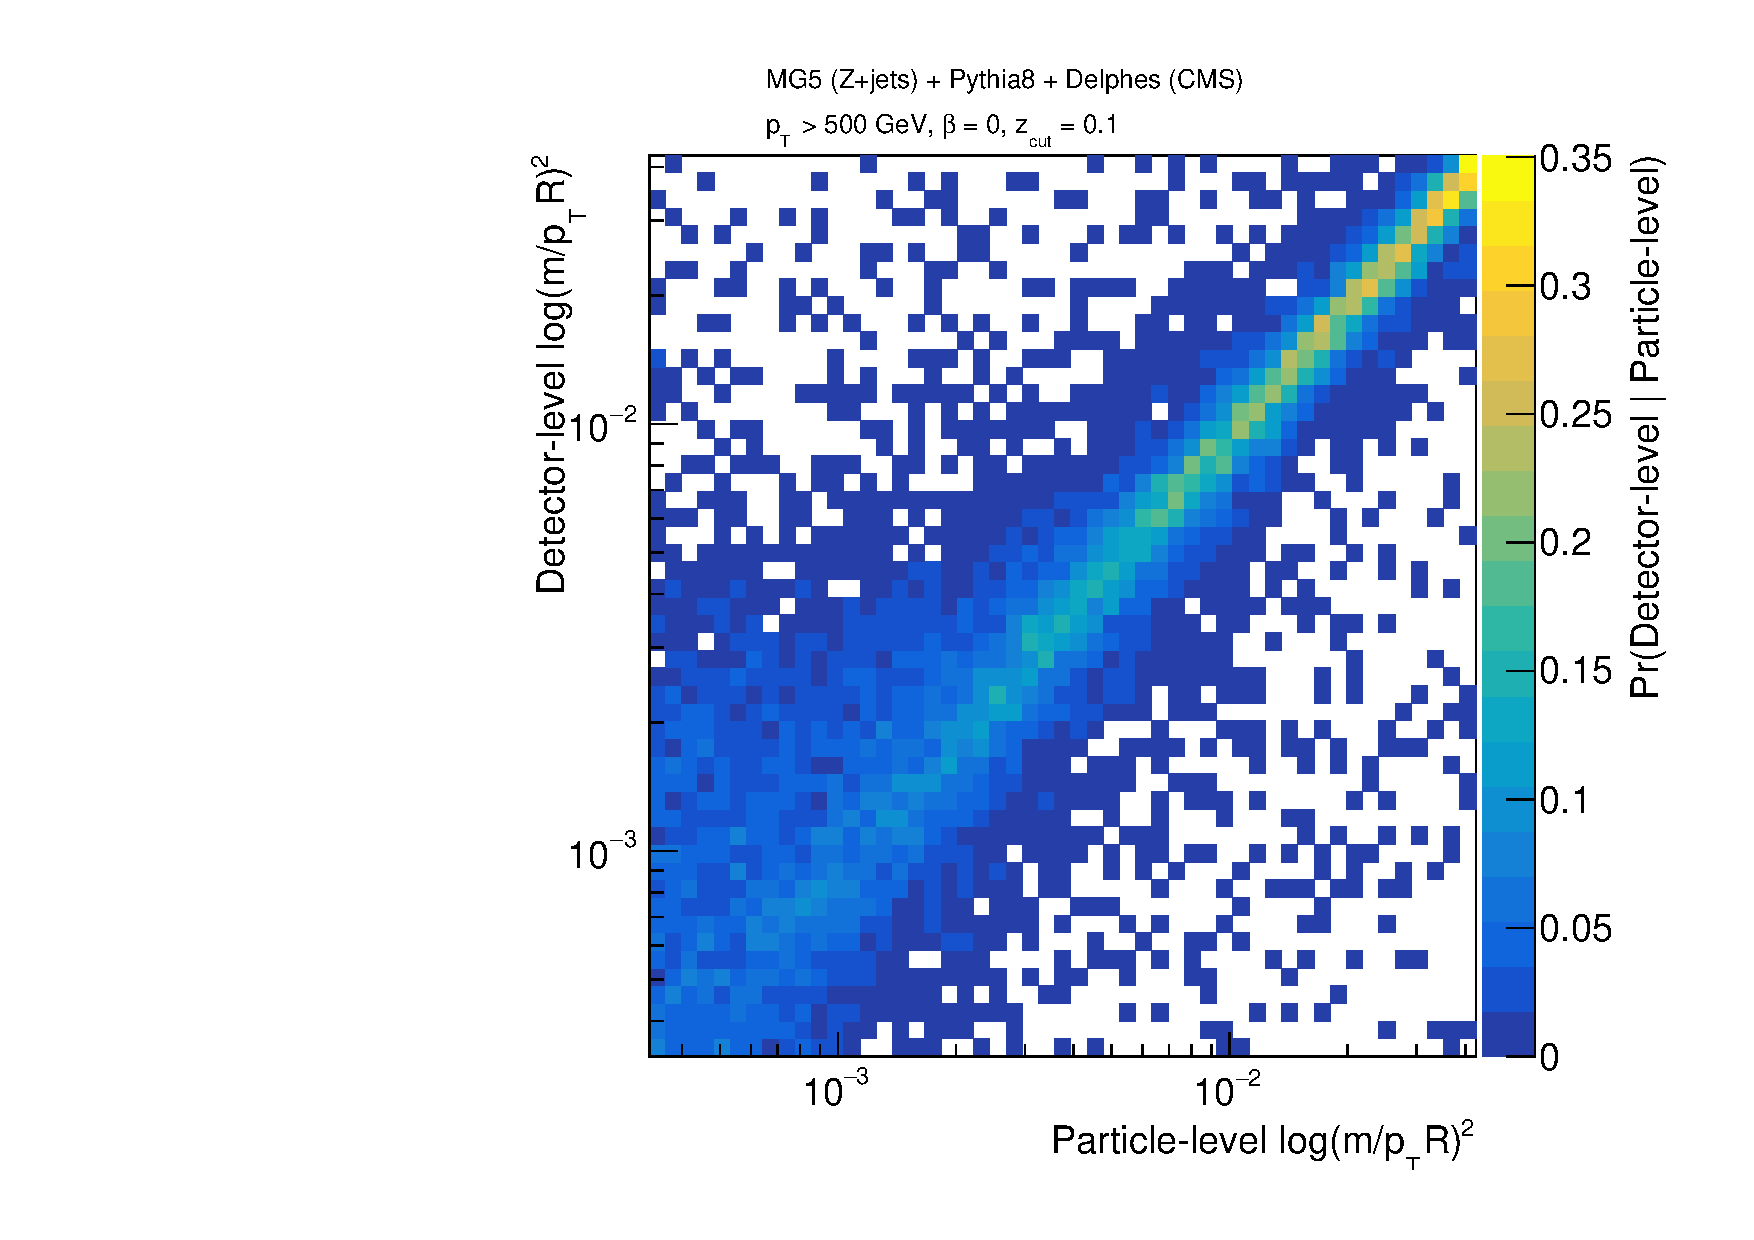
\includegraphics[width = 0.49\columnwidth]{figures/SD_resolution.pdf}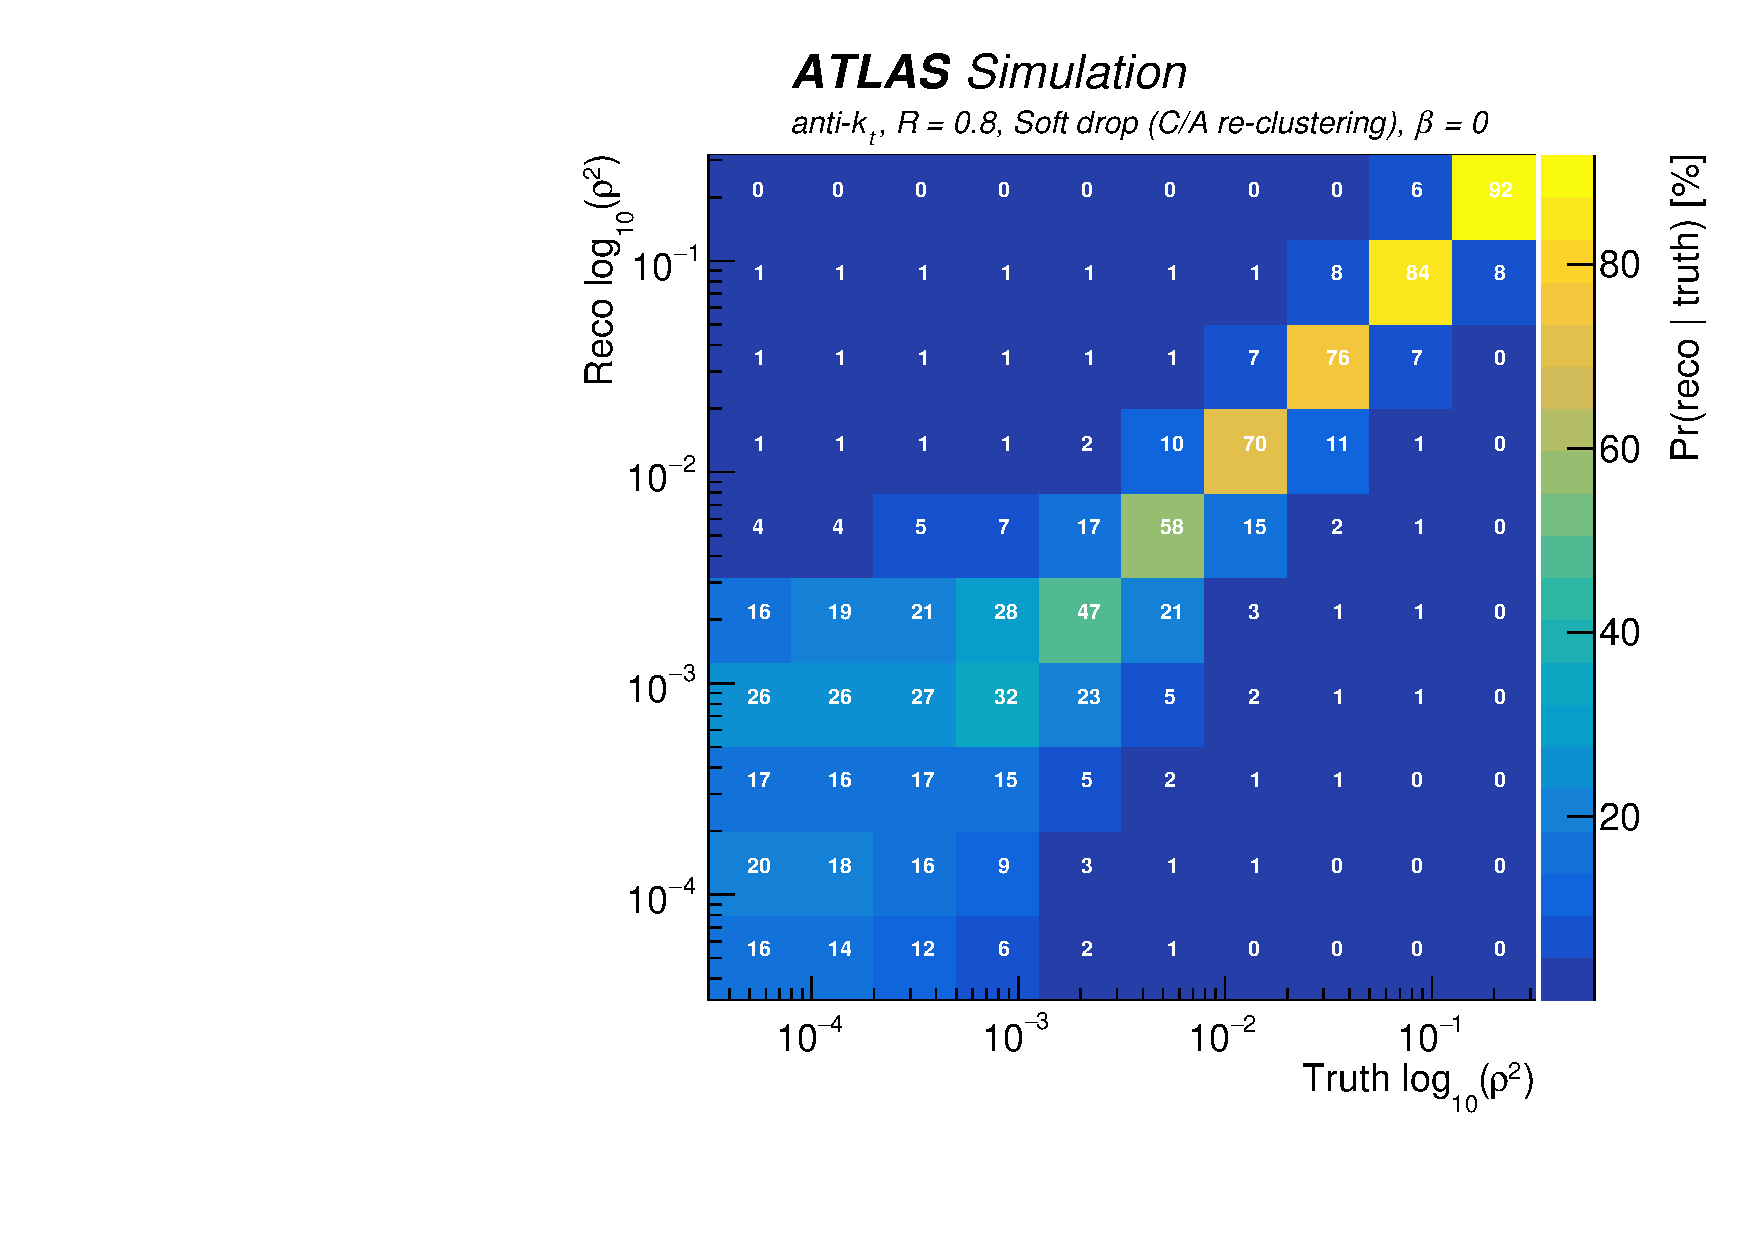
\includegraphics[width = 0.49\columnwidth]{figures/figaux_03a.pdf}
\end{center}
\caption{Left: Delphes simulation; Right: Reproduced from Ref.~\cite{Aaboud:2017qwh}.}
\label{fig:expres}
\end{figure}

\begin{figure}
\begin{center}
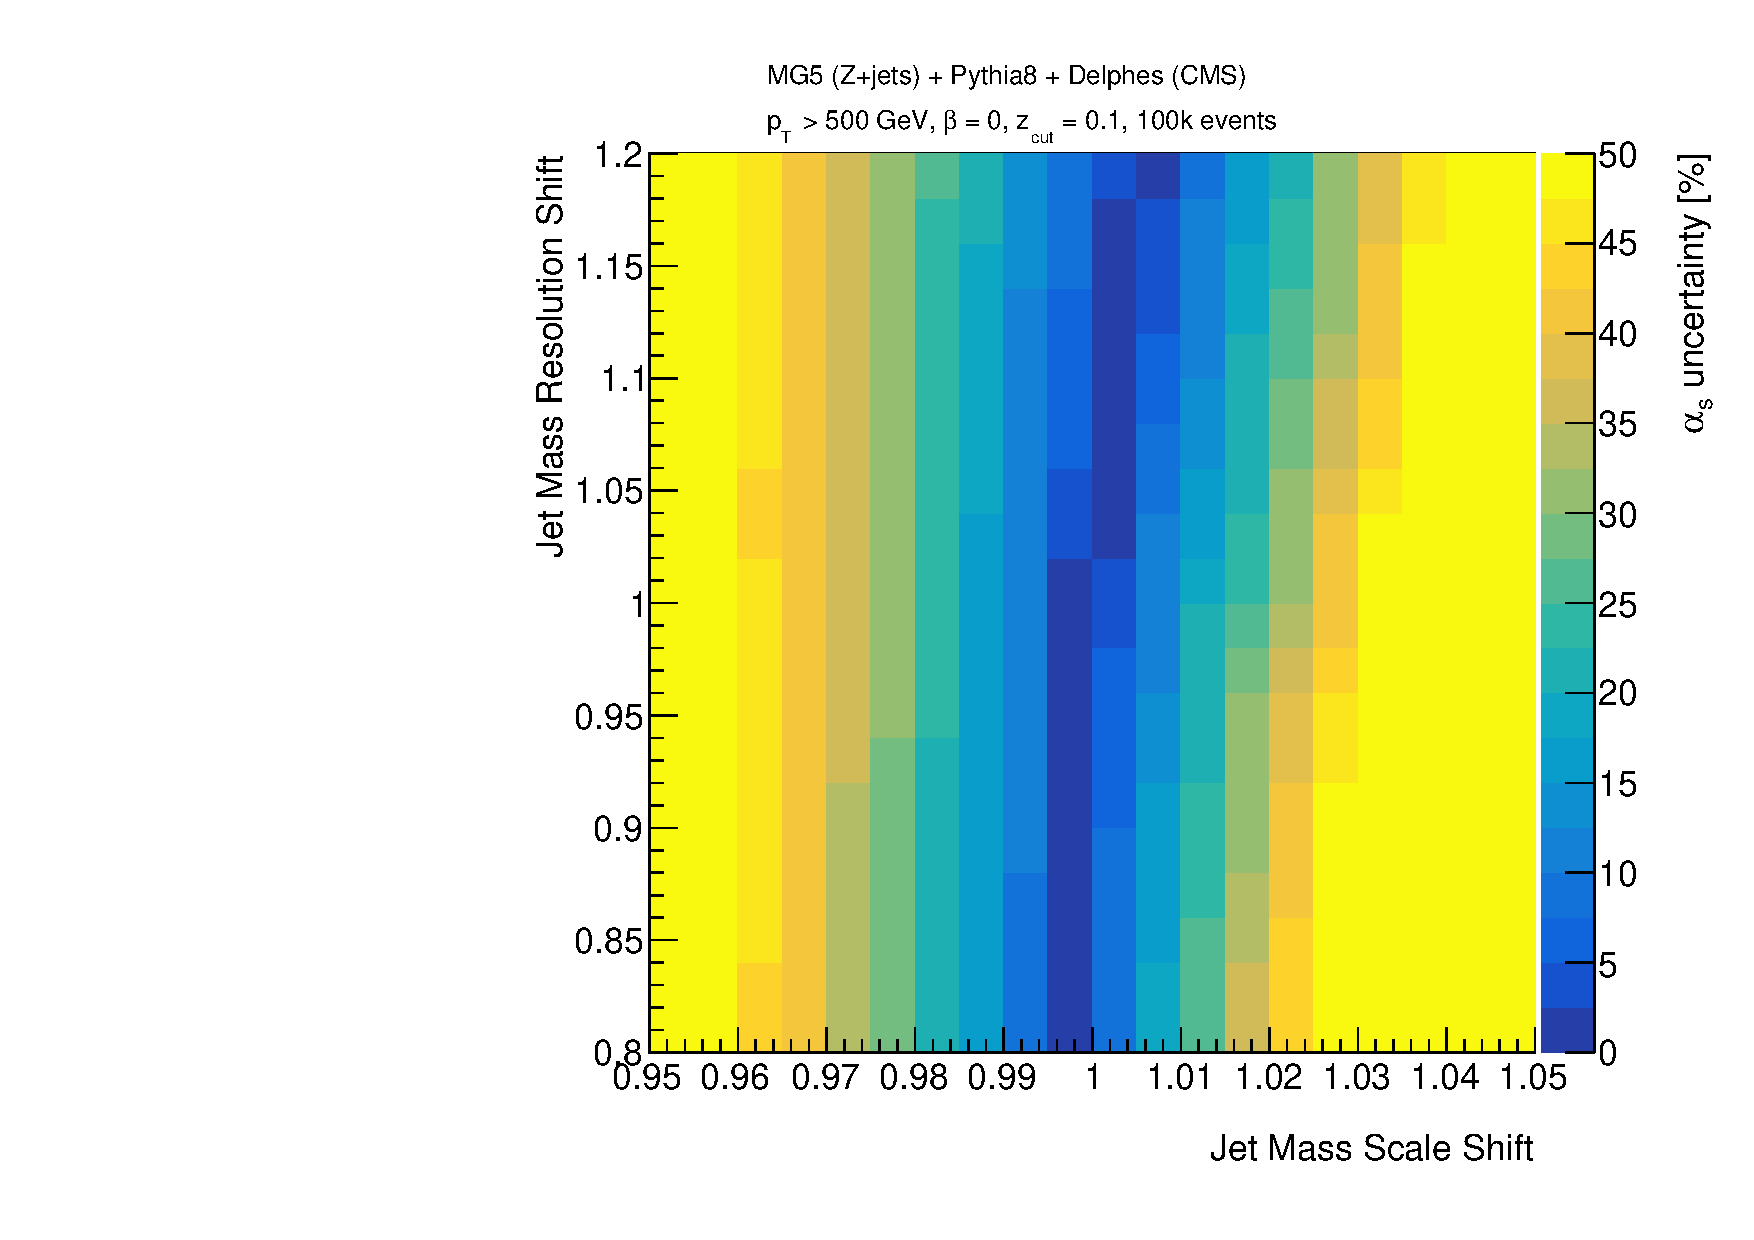
\includegraphics[width = 0.49\columnwidth]{figures/experimentaldemo/resolution_scan.pdf}
\end{center}
\caption{blah blah}
\label{fig:expfit}
\end{figure}



\subsection{Fit in Pure Quark/Gluon Samples}

Fit Methodology:
	Which fix range (minimizing theory and experimental uncertainties)?
	Constraining quark vs gluon fraction (varying SD parameters)?
	Zeroth-order feasibility study
	
	Plot is for distribution folded over PDFs (can we get rid of that?)

	Choice of jet radius (varying resummation scale)

Assume (for this section) limited by experimental uncertainties



\subsection{Constraining Quark/Gluon Fraction with Data}

	Question:  constrain quark/gluon fraction (adjust $z_cut$)?
	Need to decide beta and zcut values
	Need to matching to fixed order
	beta = 0 mass is baseline
	
	
	Another study to mitigate quark/gluon fraction uncertainties
	Sensitivitity to PDF only to the extent of getting quark/gluon fraction
	Can mitigate that with fit.


